\section{Normally distributed pseudo-random numbers}

\paragraph{a}
In Exercise 1, we are asked to write a random number generator that returns a floating point number between 0 and 1. At minimum it should be a combination of a multiply-with-carry (MWC) and a 64-bit XOR-shift. The random number generator is and plots to test its quality are given by the code snippet below.

\lstinputlisting[linerange={0-112}]{question1.py}

This script produces the following outputs:
\lstinputlisting[language={}]{q1output.txt}

Our script produces the following figures, see Figure \ref{fig:fig1}, Figure \ref{fig:fig2} and Figure \ref{fig:fig3}. From these figures, we see that the random number generator performs quite well. No clear pattern is shown in Figure \ref{fig:fig1} or in Figure \ref{fig:fig2}. The histogram in Figure \ref{fig:fig3} of the million random numbers generated looks uniform too.

\begin{figure}[ht]
\centering
\begin{minipage}[t]{.5\textwidth}
  \centering
  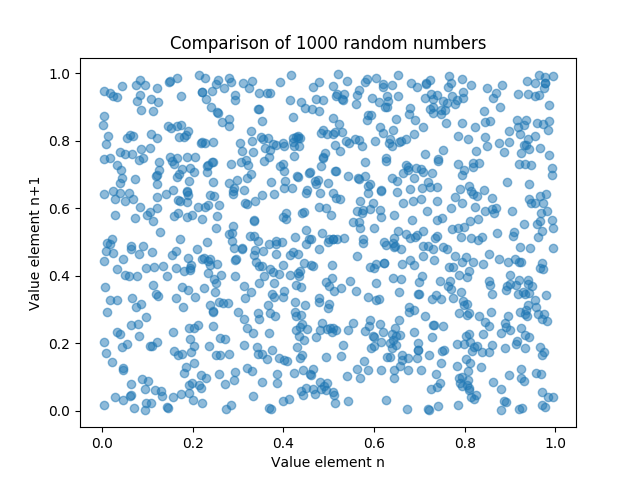
\includegraphics[width=1.0\linewidth]{./plots/q1a1.png}
  \captionsetup{width=0.8\linewidth}
  \captionof{figure}{Comparison of the first 1000 random numbers of our random number generator.}
  \label{fig:fig1}
\end{minipage}%
\begin{minipage}[t]{.5\textwidth}
  \centering
  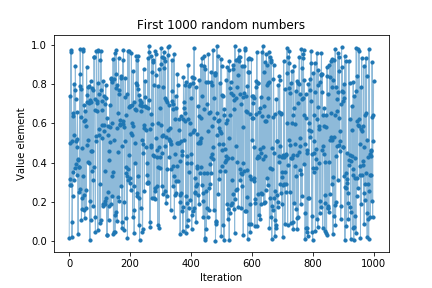
\includegraphics[width=1.0\linewidth]{./plots/q1a2.png}
  \captionsetup{width=0.8\linewidth}
  \captionof{figure}{Value of the first 1000 random numbers versus the index.}
  \label{fig:fig2}
\end{minipage}
\end{figure}

\begin{figure}[ht]
    \centering
    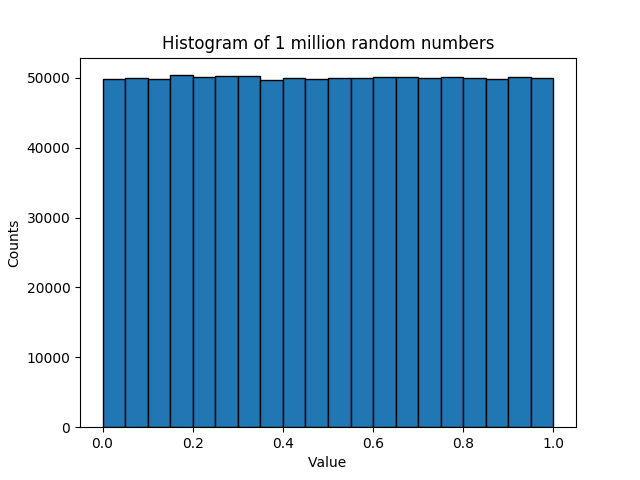
\includegraphics[width=0.5\textwidth]{./plots/q1a3.png}
    \caption{Histogram of 1 million random numbers.}
    \label{fig:fig3}
\end{figure}



\paragraph{b}
Now we use the Box-Muller method to generate 1000 normally distributed random numbers. The Box-Muller method is a very straightforward transformation from two uniformly random numbers $z_1$ and $z_2$ to two normally distributed random numbers $x_1$ and $x_2$. It is defined by
\begin{equation}
\begin{split}
    x_1 = \sqrt{-2\log(z_1)} \cos(2\pi z_2) \\
    x_2 = \sqrt{-2\log(z_1)} \sin(2\pi z_2).
\end{split}
\end{equation}

The code that does what is asked in question 1b is given below.
\lstinputlisting[linerange={112-180}]{question1.py}

Our script produces a single figure, Figure \ref{fig:fig4}. It is clear that the Box-Muller transformation and the transformation to a Gaussian with different mean and variance was successful, as the analytical function agrees very well with the histogram.

\begin{figure}[ht]
    \centering
    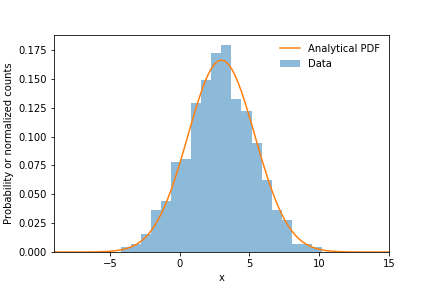
\includegraphics[width=0.5\textwidth]{./plots/q1b1.png}
    \captionsetup{width=0.8\textwidth}
    \caption{Theoretical probability distribution overlaid on the generated 1000 normally distributed random numbers with $\mu=3$ and $\sigma=2.4$.}
    \label{fig:fig4}
\end{figure}


\paragraph{c,d,e}
In question 1c, 1d and 1e we are asked to repeatedly compute the Kolmogorov Smirnov (KS) test test and Kuiper's test, be it one- or two-sample and with our own implementation or an external package. Thus we have decided to combine these questions and answer them all in the same for loop and thus piece of code. 

First, we shall give a small introduction to how we calculate the cumulative distribution function (CDF) of the standard normal distribution. The CDF of the standard normal distribution is given by
\begin{equation}
\Phi(x) = \frac{1}{\sqrt{2\pi}} \int_{-\infty}^x e^{-t^2/2} dt
\end{equation}
This can be written as 
\begin{equation}
\Phi(x) = \frac{1}{2} \left( 1+\mathrm{erf}\left(\frac{x}{\sqrt{2}} \right) \right)
\end{equation}
Where erf($x$) is the so-called the error function. It is defined as 
\begin{equation}
\mathrm{erf}(x) = \frac{2}{\sqrt{\pi}} \int_{0}^x e^{-t^2} dt
\end{equation}
We calculate this error function by means of Romberg integration.

We calculate the empirical CDF (ECDF) by sorting the data points. When the data points are sorted the index of the datapoint divided by $N$ is simply the value of the ECDF. Because we are interested in either the maximum deviation above or below, we also shift this index by one in the code, to make sure we compare the difference between both edges of each ECDF bin (see e.g., line 117-122 below). For the sorting we use our implementation of Quicksort and the \textit{argsort} implementation of Quicksort, also given below.

For Kuiper's test, we use the formula for the asymptotic distribution of the Kuiper's statistic $V$ from the Numerical Recipes book \citep{Press:2007:NRE:1403886}. Here $Q_{KP}$ is defined as

\begin{equation}
Q_{KP}(\lambda) = 2\sum_{j=1}^{\infty} (4j^2\lambda^2-1)e^{-2j^2\lambda^2}.
\end{equation}
This the value of this function is 1, to 7 figures for $\lambda < 0.4$, so we hard-code the function to return this. The $p$-value for Kuiper's test is given in terms of this function as
\begin{equation}
p = Q_{KP} \left( [\sqrt{N} + 0.155 +0.24/\sqrt{N}]V\right)
\end{equation}
where $V$ is the Kuiper's test statistic and $N$ the number of samples.



A note we should make is that the \textit{Scipy} and \textit{Astropy} functions ask for user-supplied functions to calculate the CDF (\textit{Scipy} has a built-in standard normal CDF too, but Astropy does not). For this user-supplied function we define a lambda function that simply returns the CDF values we have already calculated for our own KS-test, since this prevents the modules from doing the calculation of the CDF again.

The code we use to calculate all the required information for question 1c, 1d and 1e is given below.

\lstinputlisting[firstline=182]{question1.py}


The script outputs quite a few figures. We will start with the figures relevant to question 1c. Figure \ref{fig:fig5} shows the output of the KS test on the random numbers we have generated as a function of the number of points that we have used. We can conclude that the numbers are consistent with a normal distribution since $p>0.05$. Figures \ref{fig:fig6} and \ref{fig:fig7} show that the results of our KS test match the results of the KS test implemented in \textit{Scipy}, except for the calculation of the $p$-value for a low number of data points. This is because the series that we have used to calculate the CDF of the KS-distribution is asymptotically accurate as the number of samples becomes large. At low number of samples it performs quite well too, but this is what causes the difference with the p-values from \textit{Scipy} at a low number of points. We can see that the statistic matches perfectly, and the p-value for more than 50 data points matches very well too. 

For question 1d, Figures \ref{fig:fig8}, \ref{fig:fig9} and \ref{fig:fig10} are relevant. We see that like the KS test, Kuiper's test concludes that the numbers are indeed drawn from a standard normal distribution and our implementation of Kuiper's Test agrees very well with \textit{Astropy}. 

For question 1e, we use the two sample Kuiper's and KS test. Figures \ref{fig:fig101} to \ref{fig:fig19} show the $p$-values for data stream 0 to 9. Above the figure we indicate which set the figure corresponds to and the final $p$-values of the KS and Kuiper's test on the entire set of data points.
For most sets, we can see that the $p$-value drops very low (basically to 0) for $>10^3$ data points, calculated with both the 2 sample KS test and the 2 sample Kuiper's test. The only two sets that are interesting are set 3 and set 5. However, when considering the full extent of set 5, the resulting $p$-value also indicates that it is inconsistent with a standard normal distribution. The only set with a $p$-value above the often used threshold of 0.05 is set 3 (the fourth set, Fig. \ref{fig:fig14}). Thus we can conclude that all data sets except set 3 are inconsistent with our own Gaussian random numbers with $\sigma=1$ and $\mu=0$ and that set 3 is consistent with Gaussian random numbers with $\sigma=1$ and $\mu=0$.

\begin{figure}[ht]
\centering
\begin{minipage}[t]{.5\textwidth}
  \centering
  \includegraphics[width=1.0\linewidth]{./plots/q1c1.png}
  \captionsetup{width=0.8\linewidth}
  \captionof{figure}{KS test $p$-value of the random numbers we generated compared with the standard normal CDF.}
  \label{fig:fig5}
\end{minipage}%
\begin{minipage}[t]{.5\textwidth}
  \centering
  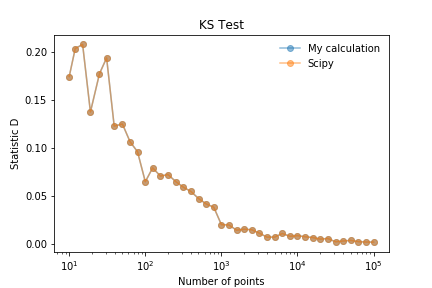
\includegraphics[width=1.0\linewidth]{./plots/q1c2.png}
  \captionsetup{width=0.8\linewidth}
  \captionof{figure}{KS test statistic D of the random numbers we generated compared with the standard normal CDF. The orange line shows the values from the \textit{Scipy} module.}
  \label{fig:fig6}
\end{minipage}
\end{figure}


\begin{figure}[ht]
\centering
\begin{minipage}[t]{.5\textwidth}
  \centering
  \includegraphics[width=1.0\linewidth]{./plots/q1c3.png}
  \captionsetup{width=0.8\linewidth}
  \captionof{figure}{KS test $p$-value of the random numbers we generated compared with the standard normal CDF. The orange line shows the values from the \textit{Scipy} module.}
  \label{fig:fig7}
\end{minipage}%
\begin{minipage}[t]{.5\textwidth}
  \centering
  \includegraphics[width=1.0\linewidth]{./plots/q1d1.png}
  \captionsetup{width=0.8\linewidth}
  \captionof{figure}{Kuiper's test $p$-value of the random numbers we generated compared with the standard normal CDF.}
  \label{fig:fig8}
\end{minipage}
\end{figure}

\begin{figure}[ht]
\centering
\begin{minipage}[t]{.5\textwidth}
  \centering
  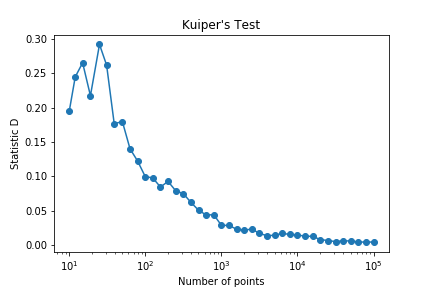
\includegraphics[width=1.0\linewidth]{./plots/q1d2.png}
  \captionsetup{width=0.8\linewidth}
  \captionof{figure}{Kuiper's test statistic $V$ of the random numbers we generated compared with the standard normal CDF. The orange line shows the values from the \textit{Astropy} module.}
  \label{fig:fig9}
\end{minipage}%
\begin{minipage}[t]{.5\textwidth}
  \centering
  \includegraphics[width=1.0\linewidth]{./plots/q1d3.png}
  \captionsetup{width=0.8\linewidth}
  \captionof{figure}{Kuiper's test $p$-value of the random numbers we generated compared with the standard normal CDF. The orange line shows the values from the \textit{Astropy} module.}
  \label{fig:fig10}
\end{minipage}
\end{figure}


%%%%%% ALL PLOTS FOR Q1e, fig 11 to 19

\begin{figure}[ht]\centering
\begin{minipage}[t]{.5\textwidth}
\centering
\includegraphics[width=1.0\linewidth]{./plots/q1e0.png}
\captionsetup{width=0.8\linewidth}
\captionof{figure}{Result of the two sample tests on the datastream indicated above the figure.}
\label{fig:fig101}
\end{minipage}%
\begin{minipage}[t]{.5\textwidth}
\centering
\includegraphics[width=1.0\linewidth]{./plots/q1e1.png}
\captionsetup{width=0.8\linewidth}
\captionof{figure}{Result of the two sample tests on the datastream indicated above the figure.}
\label{fig:fig11}
\end{minipage}%
\end{figure}

\begin{figure}[ht]\centering
\begin{minipage}[t]{.5\textwidth}
\centering
\includegraphics[width=1.0\linewidth]{./plots/q1e2.png}
\captionsetup{width=0.8\linewidth}
\captionof{figure}{Result of the two sample tests on the datastream indicated above the figure.}
\label{fig:fig12}
\end{minipage}%
\begin{minipage}[t]{.5\textwidth}
\centering
\includegraphics[width=1.0\linewidth]{./plots/q1e3.png}
\captionsetup{width=0.8\linewidth}
\captionof{figure}{Result of the two sample tests on the datastream indicated above the figure.}
\label{fig:fig13}
\end{minipage}%
\end{figure}

\begin{figure}[ht]\centering
\begin{minipage}[t]{.5\textwidth}
\centering
\includegraphics[width=1.0\linewidth]{./plots/q1e4.png}
\captionsetup{width=0.8\linewidth}
\captionof{figure}{Result of the two sample tests on the datastream indicated above the figure.}
\label{fig:fig14}
\end{minipage}%
\begin{minipage}[t]{.5\textwidth}
\centering
\includegraphics[width=1.0\linewidth]{./plots/q1e5.png}
\captionsetup{width=0.8\linewidth}
\captionof{figure}{Result of the two sample tests on the datastream indicated above the figure.}
\label{fig:fig15}
\end{minipage}%
\end{figure}

\begin{figure}[ht]\centering
\begin{minipage}[t]{.5\textwidth}
\centering
\includegraphics[width=1.0\linewidth]{./plots/q1e6.png}
\captionsetup{width=0.8\linewidth}
\captionof{figure}{Result of the two sample tests on the datastream indicated above the figure.}
\label{fig:fig16}
\end{minipage}%
\begin{minipage}[t]{.5\textwidth}
\centering
\includegraphics[width=1.0\linewidth]{./plots/q1e7.png}
\captionsetup{width=0.8\linewidth}
\captionof{figure}{Result of the two sample tests on the datastream indicated above the figure.}
\label{fig:fig17}
\end{minipage}%
\end{figure}

\begin{figure}[ht]\centering
\begin{minipage}[t]{.5\textwidth}
\centering
\includegraphics[width=1.0\linewidth]{./plots/q1e8.png}
\captionsetup{width=0.8\linewidth}
\captionof{figure}{Result of the two sample tests on the datastream indicated above the figure.}
\label{fig:fig18}
\end{minipage}%
\begin{minipage}[t]{.5\textwidth}
\centering
\includegraphics[width=1.0\linewidth]{./plots/q1e9.png}
\captionsetup{width=0.8\linewidth}
\captionof{figure}{Result of the two sample tests on the datastream indicated above the figure.}
\label{fig:fig19}
\end{minipage}%
\end{figure}
